\documentclass[11pt]{article}
\usepackage[utf8]{inputenc}
%\usepackage[latin1]{inputenc}
\usepackage[spanish]{babel}
\decimalpoint
\usepackage{anysize}
\usepackage{graphicx} 
\usepackage{amsmath}
\usepackage{booktabs}
\usepackage{tabulary}
\usepackage{nccmath}
\usepackage{float}
\usepackage{tikz}
\usetikzlibrary{patterns}
\usetikzlibrary{decorations.markings}
\usepackage{pgfplots}
\usepackage{etex}
\usepackage{color}
\usepackage{listings}
\DeclareGraphicsExtensions{.pdf,.png,.jpg}
\renewcommand{\arraystretch}{1.5}
\lstset{ %
language=Python,                % choose the language of the code
basicstyle=\normalsize,       % the size of the fonts that are used for the code
numbers=left,                   % where to put the line-numbers
numberstyle=\footnotesize,      % the size of the fonts that are used for the line-numbers
stepnumber=1,                   % the step between two line-numbers. If it is 1 each line will be numbered
numbersep=5pt,                  % how far the line-numbers are from the code
backgroundcolor=\color{white},  % choose the background color. You must add \usepackage{color}
showspaces=false,               % show spaces adding particular underscores
showstringspaces=false,         % underline spaces within strings
showtabs=false,                 % show tabs within strings adding particular underscores
frame=single,   		% adds a frame around the code
tabsize=4,  		% sets default tabsize to 2 spaces
captionpos=b,   		% sets the caption-position to bottom
breaklines=true,    	% sets automatic line breaking
breakatwhitespace=false,    % sets if automatic breaks should only happen at whitespace
escapeinside={\#}{)}          % if you want to add a comment within your code
}
\marginsize{1.25cm}{1.25cm}{0cm}{2cm}  
\title{Tarea 2 - Operaciones matemáticas básicas \\ Curso de Física Computacional}
\author{M. en C. Gustavo Contreras Mayén}
\date{ }
\begin{document}
\maketitle
\begin{enumerate}
\item La viscosidad cinemática $\mu_{k}$ del agua varía con la temperatura $T$ de la siguiente manera:
\begin{table}[H]
\centering
\begin{large} 
\begin{tabulary}{15cm}{c | c | c | c | c | c | c | c }
$T(^\circ C)$ & $0$ & $21.1$ & $37.8$ & $54.4$ & $71.1$ & $87.8$ & $100$ \\
\midrule
$\mu_{k} (10^{-3}m^{2}/s)$ & $1.79$ & $1.13$ & $0.696$ & $0.519$ & $0.338$ & $0.321$ & $0.296$ 
\end{tabulary}
\end{large}
\end{table}
Interpolar $\mu_{k}$ para $T= 10^{\circ},30^{\circ},60^{\circ}$ y $90^{\circ}$.
\item La siguiente tabla muesta como la densidad relativa $\rho$ del aire varía con la altitud $h$. Calcula la densidad relativa del aire en $10.5$ km.
\begin{table}[H]
\centering 
\begin{large}
\begin{tabulary}{15cm}{c | c | c | c | c | c | c | c }
$h(km))$ & $0$ & $1.525$ & $3.050$ & $4.575$ & $6.10$ & $7.625$ & $9.150$ \\
\midrule
$\rho$ & $1$ & $0.8617$ & $0.7385$ & $0.6292$ & $0.5328$ & $0.4481$ & $0.3741$ 
\end{tabulary}
\end{large}
\end{table}
\item Encuentra todas las raíces positivas de las siguientes ecuaciones mediante el método de bisección, con una tolerancia de 0.001.
\begin{enumerate}\label{grupo1}
\renewcommand{\arraystretch}{1.5}
\item $\tan(x) - x + 1 = 0; \hspace{1cm} 0 < x < 3\pi$
\item $\sin(x) - 0.3 \exp(x) = 0; \hspace{1cm} x > 0$
\item $-x^{3} + x + 1 = 0$
\item $16x^{5} - 20x^{3} + x^{2} + 5x - 0.5 = 0$
\end{enumerate}
\item Determina las raíces de las siguientes ecuaciones mediante el método de la falsa posición modificada:
\begin{enumerate}
\renewcommand{\arraystretch}{1.5}
\item $f(x) = 0.5\exp(\frac{x}{3})- \sin(x); \hspace{1cm} x > 0$
\item $g(x) = \log(1 + x) - x^{2}$
\item $f(x) = \exp(x) - 5x^{2}$
\item $h(x) = x^{3} + 2x - 1 = 0$
\item $f(x) = \sqrt{x+2}$
\end{enumerate}
\item Encuentra las raíces de las ecuaciones del problema (\ref{grupo1}) mediante el método de Newton-Raphson, con una tolerancia de $0.0001$
\item Identifica el intervalo para las raíces de las siguientes ecuaciones y calcula despúes las raíces mediante el método de la secante, con una tolerancia de $0.001$:
\begin{enumerate}
\item $0.1 x^{3} - 5 x^{2} - x + 4 + \exp(-x) = 0 $
\item $\ln(x) -0.2 x^{2} + 1 = 0$
\item $x + \dfrac{1}{(x+3)x}= 0$
\end{enumerate}
% \item Considera la siguiente imagen:
% \begin{figure}[H]
% \centering
% 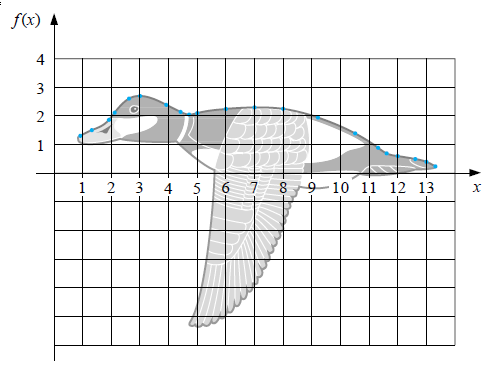
\includegraphics[scale=0.75]{Imagenes/ContornoPato.png} 
% \end{figure}
% Lo que hay que encontrar es una función que represente el contorno del pato en el primer cuadrante, para ello debes:
% \begin{enumerate}
% \item Definir un conjunto de puntos (entre 15-20 puntos)
% \item Usar la técnica de interpolación de Lagrange para revisar si la función de interpolación, representa debidamente el contorno.
% \item Usar la técnica de interpolación con splines.
% \end{enumerate}
% Discute tus resultados.
\item Usando una aproximación por diferencias finitas de orden $O(h^{2})$, calcula $f'(2.36)$ y $f''(2.36)$, a partir de los datos:
\begin{center}
\begin{tabular}{c | c | c | c | c}
x & 2.36 & 2.37 & 2.38 & 2.39 \\ \hline
f(x) & 0.85866 & 0.86289 & 0.86710 & 0.87129
\end{tabular}
\end{center}
\item Dados los siguientes datos
\begin{center}
\begin{tabular}{c | c | c | c | c | c }
x & 0.84 & 0.92 & 1.00 & 1.08 & 1.16 \\ \hline
f(x) & 0.431711 & 0.398519 & 0.367879 & 0.339596 & 0.312486
\end{tabular}
\end{center}
Calcula $f''(1)$ con la mayor precisión posible.
\item La palanca AB de longitud $R=90$ mm está girando con velocidad angular constante $d\theta/dt= 5000$ rev/min.
\begin{center}
\begin{tikzpicture}[font=\small, scale=1.4, fill=]
\draw (-0.4,-0.3) [pattern= north east lines] rectangle (0.6,0);
\draw (-0.1,0) -- node [above left]{A} (-0.1,0.3)arc (180:0:0.2cm) -- (0.3,0);
\draw (0.1,0.3) circle (0.05);
\draw [dashed] (0.1,0.3) -- node [midway, below] {x} (3.3,0.3);
\draw (3.3,0.3) circle (0.05);
\draw (1.15,1.45) circle (0.05);
\draw (0.1,0.49) -- node [midway, above] {R}(1,1.42);
\draw (0.27,0.4) -- (1.18,1.32);
\draw (1,1.42) -- (3.35,0.15) [rotate=-120] arc  (0:180:0.1cm);
\draw (3.47,0.31) -- node[midway, above, sloped]{2.5R}(1.1,1.6) [rotate=60] arc (0:180:0.1cm);
\draw (1,1.9) node {B};
\draw (2.8,-0.2) [pattern= north east lines] rectangle (4.5,-0.1);
\draw (3.05,0.65) [pattern= north east lines] rectangle (4.5,0.55);
\draw [thick] (3.1,0.3) -- (3.1,-0.07) -- (4.3,-0.07) -- node [midway, right]{C}(4.3,0.55) -- (3.1,0.55);
\draw [thick] (3.8,-0.07) -- (3.8,0.55);
\draw [thick] (3.9,-0.07) -- (3.9,0.55);
\draw [thick] (4,-0.07) -- (4,0.55);
\draw (0.5,0.3) arc (0:70:0.2cm);
\draw (0.7,0.5) node {$\theta$};
\end{tikzpicture}
\end{center}
La posición del pistón C como se muestra, varía con el ángulo $\theta$
\[x = R \left( \cos \theta + \sqrt{2.5^{2} - \sin^{2} \theta} \right)\]
Escribe un programa en python que calcule mediante diferenciación numérica la aceleración del pistón en $\theta= 0^{\circ}, 5^{\circ}, 10^{\circ},\ldots, 180^{\circ}$.
\item Las estaciones de radar \textit{A} y \textit{B} están separadas por una distancia $a=500$ m; rastrean el avión \textit{C} registrando los ángulos $\alpha$ y $\beta$ en intervalos de un segundo. Si hay tres lecturas sucesivas
\begin{center}
\begin{tabular}{c l l l }
t(s) & 9 & 10 & 11 \\ \hline
$\alpha$ & $54.80^{\circ}$ & $54.06^{\circ}$ & $53.34^{\circ}$ \\ \hline
$\beta$ & $65.59^{\circ}$ & $64.59^{\circ}$ & $63.62^{\circ}$
\end{tabular}
\end{center}
\begin{figure}[H]
	\centering
	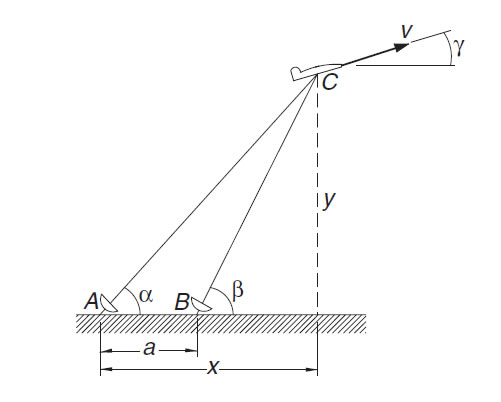
\includegraphics[scale=0.6]{Imagenes/ExamenFinal02_01.jpg} 
	\caption{Estaciones de radar y el avión.}
\end{figure}
Calcula la velocidad $v$ del avión y el ángulo de subida $\gamma$ en $t=10$ segundos. Las coordenadas del avión las tomamos de
\[x = a \dfrac{\tan \beta}{tan \beta - tan \alpha} \hspace{1.5cm} y= a\dfrac{tan \alpha \tan \beta}{\tan \beta - \tan \alpha}\]
\item Obtén la aproximación por diferencias centrales de $f''(x)$ de orden $O(h^{4})$ aplicando la extrapolación de Richardson a la aproximación por diferencias centrales de orden $O(h^{2})$.
\item Obtén la primera aproximación por diferencias centrales para $f^{4}(x)$ a partir de la serie de Taylor.
\item Usa la regla del trapecio recursiva para evaluar
\[ \int_{0}^{\frac{\pi}{4}} ln(1 + \tan(x)) dx\]
Explica tus resultados.
\item La siguiente tabla indica la potencia $P$ propocionada por las ruedas de un carro como función de la velocidad $v$. Si la masa del carro es $m=2000$ kg, calcula el tiempo $\Delta t$ necesario para que el carro acelere de $1$ m/s a $6$ m/s. Usa la regla del trapecio para integrar. Tip:
\[ \Delta t = m \int_{1s}^{6s} \left( \dfrac{v}{P} \right) dv\]
que se puede obtener de la ley de Newton $F= m/(dv/dt)$ y por la definición de potencia, $P=Fv$.
\begin{center}
\begin{tabular}{c | c | c | c | c | c | c | c | c}
$v$ (m/s) & 0 & 1.0 & 1.8 & 2.4 & 3.5 & 4.4 & 5.1 & 6.0 \\ \hline
$P$ (kW)  & 0 & 4.7 & 12.2 & 19.0 & 31.8 & 40.1 & 43.8 & 43.2 
\end{tabular}
\end{center}
\item La siguiente tabla proporciona el empuje $F$ del arco como función del desplazamiento $x$. Si la cuerda tiene un desplazamiento de $0.5$ m, calcula la velocidad de una flecha de $0.075$ kg, cuando sale del arco. Tip: la energía cinética de la flecha es igual al trabajo hecho al estirar la cuerda, que es:
\[ m \dfrac{v^{2}}{2} = \int_{0}^{0.5m} F dx\]
\begin{center}
\begin{tabular}{c | c | c | c | c | c | c |}
$x$ (m) & 0.00 & 0.05 & 0.10 & 0.15 & 0.20 & 0.25  \\ \hline
$F$ (N)  & 0 & 37 & 71 & 104 & 134 & 161
\end{tabular}
\end{center}
\begin{center}
\begin{tabular}{c | c | c | c | c | c | }
$x$ (m) & 0.30 & 0.35 & 0.40 & 0.45 & 0.50 \\ \hline
$F$ (N)  & 185 & 207 & 225 & 239 & 250 
\end{tabular}
\end{center}
\begin{figure}[H]
	\centering
	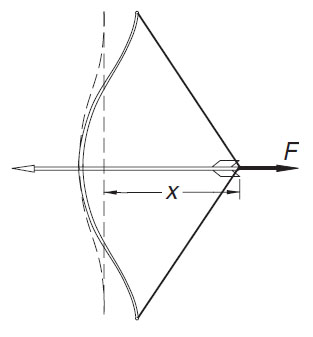
\includegraphics[scale=0.5]{Imagenes/Integral_01_Arco.jpg} 
	\caption{Flecha para el ejercicio}
\end{figure}
\item El período de un péndulo de longitud $L$ es $\tau = 4 \sqrt{\frac{L}{g}} h(\theta_{0})$, donde $g$ es la aceleración debida a la gravedad, $\theta_{0}$, representa la amplitud angular y 
\[ h(\theta_{0}) =  \int_{0}^{\frac{\pi}{2}} \dfrac{d\theta}{\sqrt{1 - \sin^{2} \left( \frac{\theta_{0}}{2}\right) \sin^{2} \theta}} \]
Calcular $h(15^{\circ})$, $h(30^{\circ})$ y $h(45^{\circ})$; compara esos valores con $h(0^{\circ}) = \frac{\pi}{2}$ (la aproximación usada para pequeñas amplitudes)
\item La fórmula de Debye para la capacidad calorífica $C_{v}$ de un sólido, es $C_{v} = 9 Nkg(u)$, donde
\[g(u) = u^{3} \int_{0}^{1/u} \dfrac{x^{4}e^{x}}{(e^{x}-1)}dx\]
los términos de la ecuación son:
\\
\\
\begin{minipage}{4cm}
\begin{eqnarray*}
N &=& \text{Número de partículas en el sólido} \\
k &=& \text{Constante de Boltzmann} \\
u &=& \frac{T}{\Theta_{D}}
\end{eqnarray*}
\end{minipage}
\hspace{3cm}
\begin{minipage}{4cm}
\begin{eqnarray*}
T &=& \text{temperatura absoluta} \\
\Theta_{D} &=& \text{Temperatura de Debye}
\end{eqnarray*}
\end{minipage}
\\
Calcular $g(u)$ para $u=0$ a $1.0$ en intervalos de $0.05$, grafica los resultados.
\item Una masa $m$ est\'{a} unida a un resorte de longitud $b$ y rigidez $k$. Se puede demostrar que la aceleración de la masa es $\ddot{x} = -f(x)$, donde
\[f(x) = \mu g + \dfrac{k}{m} (\mu b + x) \left( 1 - \dfrac{b}{\sqrt{b^{2} + x^{2}}} \right)\]
Si la masa se libera del reposo en $x=b$, y la velocidad en $x=0$ est\'{a} dada por
\[ v_{0} = \sqrt{2 \int_{0}^{b} f(x) dx}\]
\begin{figure}[H]
	\centering
	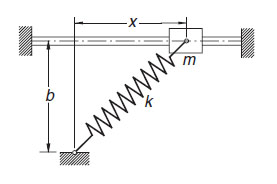
\includegraphics[scale=0.5]{Imagenes/Integral_02_Resorte.jpg}
	\caption{Masa unida a un resorte.}
\end{figure}
Calcular mediante integración numérica el valor de $v_{0}$, usando $m=0.8$ k, $b=0.4$ m, $\mu=0.3$, $k=80$ N/m y $g=9.81$ $m/s^{2}$.
\item Las integrales de Fresnel
\begin{align*}
C(w) &= \int_{0}^{w} \cos \left( \dfrac{\pi \: u^{2}}{2} \right) \: du \\[1em]
S(w) &= \int_{0}^{w} \sin \left( \dfrac{\pi \: u^{2}}{2} \right) \: du
\end{align*}
son la base de la teoría de la difracción óptica. Calcula las integrales para $-3.5 \leq w \leq 3.5$, genera una gráfica de $S(w)$ contra $C(w)$, las curvas obtenidas se les llama \textit{espiral de Cornu}.
\end{enumerate}
\end{document}